\documentclass[titlepage,oneside,final,14pt]{extarticle} % тип документа (титульник, односторонняя, финальная версия, 14 пункт по дефолту)

\usepackage[utf8]{inputenc} % кодировка
\usepackage[english,russian]{babel} % переносы и поддержка языка
\usepackage{indentfirst} % отступы в абзаце
\usepackage{vmargin}
\usepackage{hyperref} % гиперссылки
\usepackage[formats]{listings} % листинги кода
\usepackage{color} % создание цветов
\usepackage{graphicx} % картинки
\usepackage{tempora} % шрифт
\usepackage{float} % чтоб картинки не плавали [H]
\usepackage{setspace} 
\usepackage{chngcntr} 
\usepackage{ccaption} 
\usepackage{titlesec} % для заголовков
\usepackage{ragged2e} % для выравнивания по ширине
\usepackage{enumitem} % для межстрочного интервала в списках
\usepackage{seqsplit}
\usepackage{minted}

\setlist{nosep} % убирает отступы для элементов списка
\titleformat{\section}[hang]{\normalfont\Large\bfseries\filcenter}{\thesection}{1em}{}[] % настройки заголовков
\titleformat{\subsection}[hang]{\filcenter\bfseries}{\thesubsection}{1em}{}[]
\titleformat{\subsubsection}[hang]{\filcenter\bfseries}{\thesubsubsection}{1em}{}[]
\newcommand{\sectionbreak}{\clearpage} % для разрыва листа для новой секции

\RequirePackage{caption}
\DeclareCaptionLabelSeparator{defis}{ --- }
\captionsetup{justification=centering,labelsep=defis} % для тире в подписях к картинкам

\counterwithin{figure}{section} % счетчик для картинок
\onehalfspacing % полуторный интервал
\graphicspath{{./images/}} % путь к папке с картинками
\setpapersize{A4} % а4 лист
\setmarginsrb{30mm}{20mm}{15mm}{20mm}{0pt}{0mm}{0pt}{10mm} % поля - левое, верхнее, правое, нижнее

 % абзацный отступ
\sloppy % чтоб не вылезало за пределы листа

\lstdefineformat{Java}{%
	\{=\string\newline\indent,%
	\}=[;]\newline\noindent\string\newline,%
	\};=\newline\noindent\string\newline,%
	;=[\ ]\string\space}

\lstset{language=Java,
	format=Java,
	showspaces=false,
	showtabs=false,
	breaklines=true,
	showstringspaces=false,
	commentstyle=\color{pgreen},
	keywordstyle=\color{pblue},
	stringstyle=\color{pred},
	basicstyle=\linespread{1}\small\ttfamily,
	columns=fullflexible
} % настройки листинга кода

\definecolor{pblue}{rgb}{0.13,0.13,1}
\definecolor{pgreen}{rgb}{0,0.5,0}
\definecolor{pred}{rgb}{0.9,0,0}
\definecolor{pgrey}{rgb}{0.46,0.45,0.48}

\hyphenpenalty=100000 % для отсутствия переносов
\justifying % по ширине

\author{Bulychev Ivan}
\title{Лабораторная работа №1}

\begin{document}
		
\begin{titlepage}
	\begin{spacing}{1.1}
		\begin{center}		
			ФЕДЕРАЛЬНОЕ АГЕНТСТВО СВЯЗИ 
			\\
			Федеральное государственное бюджетное образовательное учреждение высшего образования
			\\
			<<ПОВОЛЖСКИЙ ГОСУДАРСТВЕННЫЙ УНИВЕРСИТЕТ ТЕЛЕКОММУНИКАЦИЙ И ИНФОРМАТИКИ>>
			\\			
			\vspace{1em}
			Факультет информационных систем и технологий
			\\
			Кафедра программного обеспечения и управления в технических системах
			\\
			\vspace{7em}
			\bfseries\Large
			ОТЧЕТ
			\\
			ПО ЛАБОРАТОРНОЙ РАБОТЕ № \underline{\hspace{0.4em}1\hspace{0.4em}}
			\\
			\vspace{0.5em}
			\normalfont
			\normalsize
			по дисциплине
			\underline{\hspace{4em}Параллельное программирование\hspace{4em}}
			\\
			\small
			\hspace{4em} название (при наличии)
			\normalsize
			\\
			\hspace{3em}			
			\underline{\hspace{3em}Запуск консольного приложения на кластере MPI\hspace{3em}}
			\\
			\small
			\hspace{4em} название работы (при наличии)
			\normalsize
			\\		
	\end{center}			
			\vspace{5em}
			\begin{minipage}{0.5\textwidth}
				\begin{flushleft}					
				\end{flushleft}
			\end{minipage}
			\begin{minipage}{0.5\textwidth}
				\begin{center}
					\bfseries
					ВЫПОЛНИЛ
					\\
					\normalfont
					студент \hspace{1ex} \underline{гр. ПО--61} \hspace{1ex} \underline{Булычев И. Д.}
					\\
					\small
					\hspace{3.5em} (группа) \hspace{3.5em} (ФИО)
					\normalsize\bfseries
					ПРОВЕРИЛА
					\\
					\normalfont
					\hspace{1ex} \underline{к. т. н., доцент} \hspace{1ex} \underline{Мезенцева Е. М.}
					\\
					\small
					(должность) \hspace{5em} (ФИО)
					\\	
					\normalfont				
				\end{center}
			\end{minipage}
		\begin{center}
			\vspace{6em}
			Самара
			\\
			2019
			\end{center}

			

\end{spacing}
\end{titlepage}
\setcounter{page}{2}
\setlength{\parindent}{1.25cm} % абзацный отступ
\section{Цель лабораторной работы}

\subsection{Цель работы}

Разработать и запустить на кластере программу на любом из языков программирования, вычисляющую число $\pi$.

\subsection{Используемое программное обеспечение}

Для выполнения лабораторной работы мною было использовано следующее программное обеспечение:
\begin{itemize}
	\item ОС Ubuntu 18.10
	\item IDE Intellij Idea 2018.3
	\item JDK 1.8
	\item MPJ Express 0.44
\end{itemize}

\section{Ход выполнения лабораторной работы}

\subsection{Формула расчета}

Для расчета числа $\pi$ используется формула Бэйли-Боруэйна-Плаффа (ББП-формула):

\begin{equation}\label{bbp}
    \pi = \sum\limits_{k=0}^{\infty} \frac{1}{16^k} \Bigg(\frac{4}{8k+1} - \frac{1}{8k+4} - \frac{1}{8k+5} - \frac{1}{8k+6} \Bigg).
\end{equation}

\subsection{Реализация вычислений}

Для получения числа $\pi$ с высокой точностью все вычисления проводятся с помощью Java-класса BigDecimal.

Для использования данного класса необходимо создать пользовательскую MPI-функцию (интерфейс MPI.User\_function) и MPI-операцию (класс mpi.Op) для использования в функции MPI.COMM\_WORLD.Reduce().

Входные данные для вычислений (количество членов ряда, количество знаков после запятой) указано в файле input.txt.

\subsubsection{Создание пользовательской функции}

Так как тип User\_function является интерфейсным, то при создании объекта данного типа необходимо переопределить метод Call, принимающий в качестве аргументов:
\begin{itemize}
	\item входной массив значений;
	\item индекс массива, начиная с которого будет применяться данная функция во входном массиве;
	\item выходной массив значений, в который записывается результат;
	\item индекс массива, начиная с которого будет записываться результат  в выходном массиве;
	\item количество элементов массивов, с которыми нужно произвести действия;
	\item тип данных, в который преобразуется выходной массив.
\end{itemize}   

В методе Call описывается операция, которая должна выполняться на соответствующих элементах входного и выходного массива с записью результата в выходной массив. В данном случае выполняется операция сложения двух чисел типа BigDecimal.

\subsubsection{Создание пользовательской операции}

Для использования функции Reduce с пользовательскими объектами, необходимо создать пользовательскую операцию. Для этого нужно создать объект типа mpi.Op. 

Параметры конструктора:
\begin{itemize}
	\item Объект пользовательской функции;
	\item Логическое значение --- является ли функция коммутативной.
\end{itemize}

\subsubsection{Функция вычисления числа $\pi$}

Число $\pi$ вычисляет функция calculatePi(). Эта функция использует формулу Бэйли-Боруэйна-Плаффа. Её входные параметры:
\begin{itemize}
	\item Начальный индекс суммы;
	\item Конечный индекс суммы;
	\item Количество знаков после запятой.
\end{itemize}

Данная функция вычисляется параллельно. Каждый процесс вычисляет сумму указанного диапазона членов ряда. 

\subsubsection{Получение конечного результата}

Для получения конечного результата вычислений --- редуцирования результатов вычислений каждого процесса --- используется функция Reduce(). Ее входные параметры:
\begin{itemize}
	\item Входной массив результатов вычисления данного процесса:
	\item Начальный индекс входного массива;
	\item Выходной массив результатов редуцирования;
	\item Начальный индекс выходного массива;
	\item Количество элементов, над которыми производится редуцирование;
	\item Тип элементов;
	\item Операция, производимая над соответствующими элементами входного и выходного массивов с записью в выходной массив;
	\item Номер процесса, в котором будет храниться финальное значение переменной.
\end{itemize}

Актуальное (финальное) значение числа $\pi$ хранится в переменной процесса 0. В остальных процессах данная переменная так же присутствует, но в ней хранятся промежуточные результаты суммирования. Поэтому для вывода числа $\pi$ на экран запрашивается значение переменной процесса 0. 

\section{Результаты выполнения лабораторной работы}

\subsection{Листинг приложения}

\begin{lstlisting}
package lab3;

import mpi.*;

import java.io.File;
import java.math.BigDecimal;
import java.math.RoundingMode;
import java.util.Scanner;

public class PiCalc {
public static void main(String[] args) throws Exception {

Scanner in = new Scanner(new File("src/lab3/input.txt"));
int scale = in.nextInt(); // precision
int iter = in.nextInt(); // iteration num

// o is an input array, o1 is a reduce array (accumulator)
User_function function = new User_function() {
@Override
public void Call(Object o, int i, Object o1, int i1, int i2, Datatype datatype) throws MPIException {
BigDecimal arg = ((BigDecimal[]) o)[0];
Object[] resultArray = ((Object[]) o1);
BigDecimal accumulator = (BigDecimal) resultArray[0];
resultArray[0] = accumulator.add(arg);
}
};
// user defined reduce operation
Op op = new Op(function, false);
BigDecimal[] res = {BigDecimal.ZERO};
MPI.Init(args);
int size = MPI.COMM_WORLD.Size(); // proc amnt
int rank = MPI.COMM_WORLD.Rank(); // proc num

// just for equal amount of iterations for each process (like (170 / 4) * 4 == 168 )
iter = ( iter / size ) * size;
int processStep = iter / size; // iter amnt for each proc
BigDecimal[] stepRes =  {BigDecimal.ZERO}; // start from zero
stepRes[0] = calculatePi(rank*processStep, (rank+1) * processStep, scale); // calculating for each process
MPI.COMM_WORLD.Reduce(stepRes, 0, res, 0, 1, MPI.OBJECT,  op, 0); // sum all in res
MPI.Finalize(); // shutting down
if (rank == 0) {
System.out.println(res[0]);
System.out.println(res[0].equals(calculatePi(0, iter, scale))); // correct check
}
}

// Bailey-Borwein-Plouffe formula
private static BigDecimal calculatePi(int start, int end, int scale) {
BigDecimal e = BigDecimal.ZERO;
for (int k = start; k < end; k++) {
BigDecimal a0 = new BigDecimal(16).pow(k);
BigDecimal a1 = new BigDecimal(4).divide(new BigDecimal(8*k+1), scale, RoundingMode.HALF_UP);
BigDecimal a2 = new BigDecimal(2).divide(new BigDecimal(8*k+4), scale, RoundingMode.HALF_UP);
BigDecimal a3 = new BigDecimal(1).divide(new BigDecimal(8*k+5), scale, RoundingMode.HALF_UP);
BigDecimal a4 = new BigDecimal(1).divide(new BigDecimal(8*k+6), scale, RoundingMode.HALF_UP);
BigDecimal a5 = a1.subtract(a2).subtract(a3).subtract(a4);
BigDecimal a6 = BigDecimal.ONE.divide(a0, scale, RoundingMode.HALF_UP);
BigDecimal elem = a5.multiply(a6);
e = e.add(elem);
}
return e;
}
}


\end{lstlisting}

\subsection{Результат выполнения}

Входные значения равны 200 и 100 (итерации и точность).

\ttfamily\small
\seqsplit{
3.1415926535897932384626433832795028841971693993751058209749445923078164062862089986280348253421170679821480865132823066470938350119627942072033649368930652918677481046443747275745835689496799830568544722349378129656839482659850525886071657298598733689069807459088463344360298382832879208231436429314344581896143365041340636074918524482183533734830644393147695032526939304802748576134091869887195597172}

true

\normalfont\normalsize

\begin{figure}[H]
	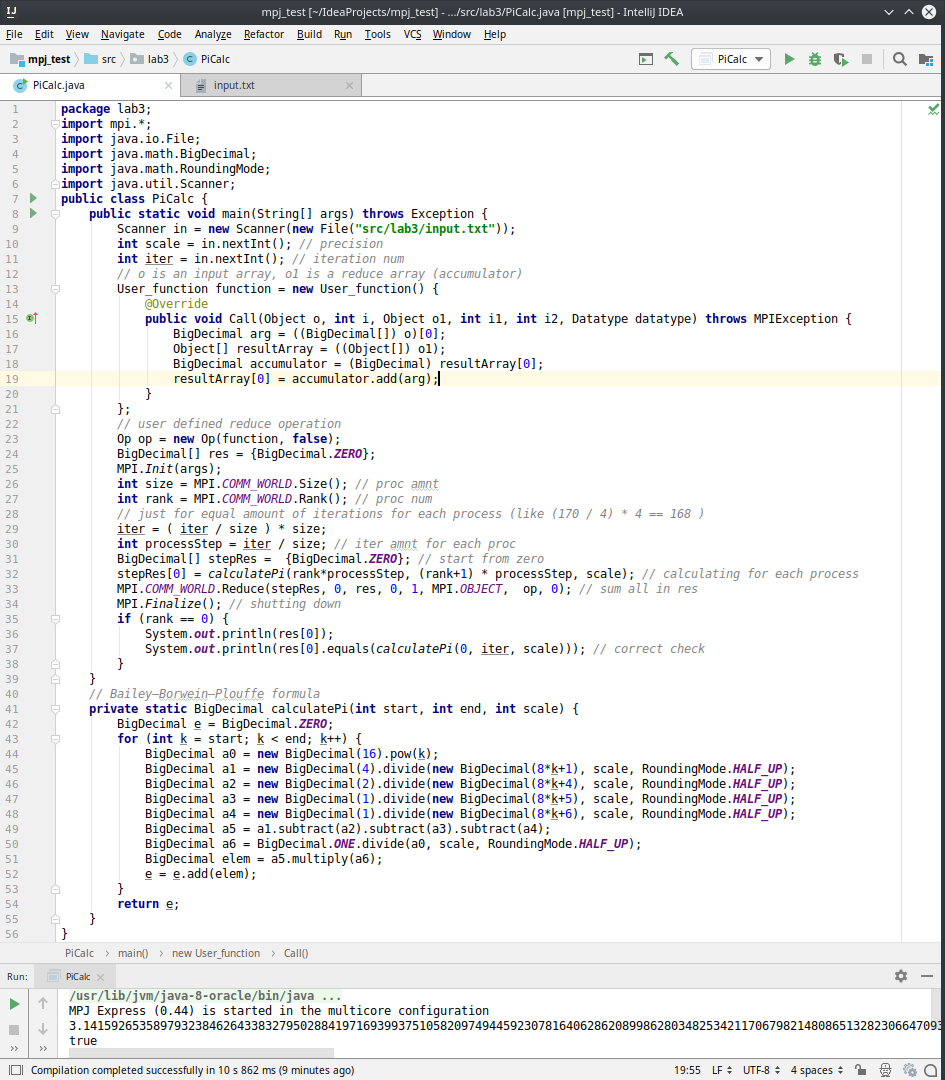
\includegraphics[width=0.9\linewidth]{code_listing_results}
	\centering
	\caption{Листинг и результат выполнения}
\end{figure}

\section{Выводы по результатам выполнения лабораторной работы}

В ходе работы была написано консольное приложение на языке Java в среде программирования Intellij Idea, к которой подключена библиотека MPJ Express. Каждый процесс
рассчитывает свои значения суммы членов ряда в заданном диапазоне, после чего выполняется суммирование промежуточных результатов с помощью функции Reduce. После чего на экран выводится значение числа $\pi$ и проверка корректности результата --- сравнение с числом $\pi$, вычисленным не параллельно.

Выполнен тестовый запуск программы на кластере, состоящем из ядер процессора компьютера.

\end{document}
